\documentclass{article}
\usepackage[T1]{fontenc}
\usepackage{lmodern}
\usepackage{graphicx}
\usepackage{amsmath,amssymb}
\usepackage[a4paper,margin=2cm]{geometry}
\usepackage[absolute,overlay]{textpos}
\setlength{\TPHorizModule}{1mm}
\setlength{\TPVertModule}{1mm}
\usepackage[indonesian]{babel}
\usepackage{hyperref}
\setlength{\emergencystretch}{2em}
% unit: Halaman 61

\begin{document}

% === Halaman 61 (llm) ===

\section*{Free Online Image steganography Encoder tool}

\vspace{163.35mm}

The image steganography tool allows you to embed hidden data inside a carrier file, such as an image. You could extract data from Free Online Image Steganographic DecoderTool .

% deskripsi: Screenshot antarmuka web tool Encoder Steganografi Gambar yang mencakup opsi untuk memilih gambar, memasukkan teks yang ingin disembunyikan, dan kolom kata sandi.
% bbox normalisasi: [0.2300, 0.3300, 0.8100, 0.8800]
\begin{textblock*}{121.80mm}(48.30mm,98.01mm)
\noindent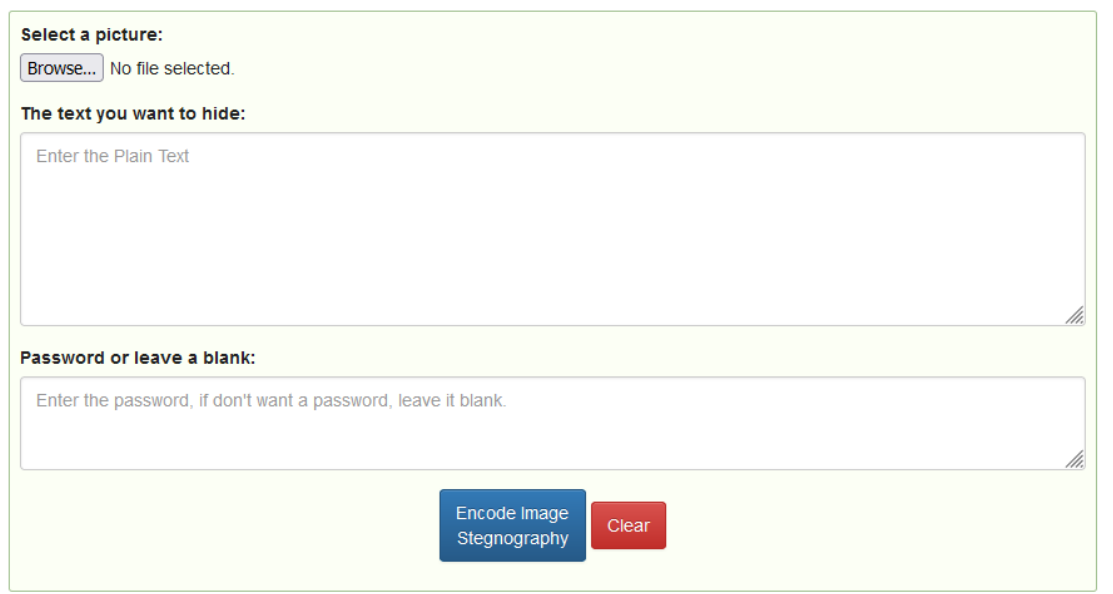
\includegraphics[width=121.80mm,height=163.35mm]{../../images/llm/page_061_img_01.png}%
\end{textblock*}

\end{document}
